%!TEX root = proposal.tex
%\addbibresource{bibliography.bib}
%----------------------------------------------------------------------------
\section{Work Completed}\label{sect:workCompleted}
%----------------------------------------------------------------------------

As part of the preliminary evaluation process, I am in the process of implementing the Galois microarchitecture 
depicted in Figure \ref{fig:uarch} with hand-written rather than compiler-generated engines for the delta-stepping 
SSSP algorithm. All hardware modules, including both Galois library modules as well as the SSSP engines, are written 
in Bluespec System Verilog \cite{bluespec}, a high-level hardware description language.
Ideally, the use of Bluespec should enable much tighter control of 
the generated Galois microarchitecture compared to HLS languages while greatly increasing productivity over hardware 
description languages like SystemVerilog.

\subsection{The Convey MX-100}

\begin{table}
\centering
\begin{tabular}{ | l | l | }
  \hline
  \textbf{Method} & \textbf{Description} \\
  \hline
  CPU & 1x Intel Xeon E5-2643 \\
  \hline
  CPU Memory & 256GB DDR3 \\
  \hline
  FPGA & 4x Virtex-6 HX-565T \\
  \hline
  FPGA Memory & 128GB SG-DIMMs \\
  \hline
  FPGA Memory Bandwidth & 128GB/s \\
  \hline
\end{tabular}
\caption{Worklist interface}
\label{table:conveySpecs}
\end{table}

\begin{figure}
\centering
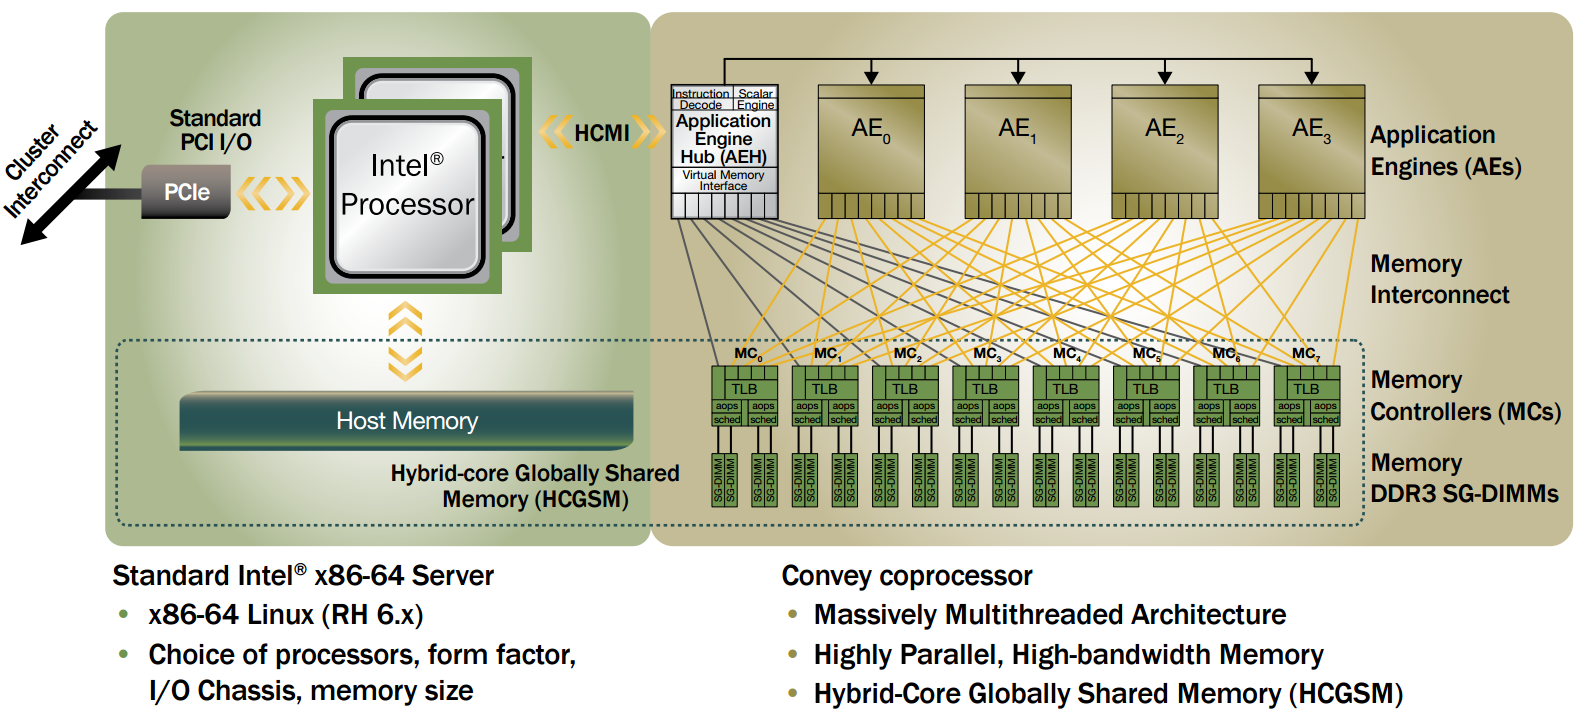
\includegraphics[width=15cm, keepaspectratio]{pics/convey.png}
\caption{Convey MX-100 architectural overview}
\label{fig:convey}
\end{figure}

I am currently targeting the Convey MX-100 as my FPGA platform. As shown in Table \ref{table:conveySpecs}, the MX-100 
is a bleeding-edge machine coupling fast general-purpose processors with multiple FPGAs with dedicated high-bandwidth 
scatter-gather memory optimized for 64-bit operations. Figure \ref{fig:convey} depicts the overall platform 
architecture. The four FPGAs, known as Application Engines, are connected with a crossbar to 8 memory controllers, 
each connecting to two channels of scatter-gather memory optimized for 64-bit random access, for a total of 16 memory 
channels. To design a Convey hybrid-core program, the engineer first designs a custom Personality, consisting of the 
FPGA bit-file containing a custom instruction set designed to accelerate individual algorithms within applications. 
The Personality source code must interface with Convey's Personality Development Kit (PDK), which presents an 
interface to Convey's abstraction layer, including its memory interface. Convey users must explicitly transfer data 
to the FPGA memory before calling the Personality instruction, and transfer the results back to CPU memory upon 
instruction completion. To run on Convey, the Galois microarchitecture resides within a Personality. The Galois HLS 
tool generates the hybrid-core program along with the required data transfers to and from FPGA memory.

The MX-100 is so far the only machine designed by Convey to support atomic memory operations, including atomic add, 
subtract, and compare-and-swap (CAS) operations. I chose the MX-100 platform because these atomic operations are 
essential for supporting high-performance synchronization across multiple FPGAs. In addition, the specialized Convey scatter-gather 
memory is perfect for supporting the pointer-chasing memory access patterns present in many Galois programs such as 
SSSP.

\subsection{Implemented Custom SSSP Engine}

\begin{figure}
\centering
\lstset{language=Java}
\begin{lstlisting}
Graph graph = { /* init */}; // Initialize graph contents
WorkList<GraphNode> workQ();
workQ.enq(init); // worklist initialized with the starting node
foreach(uint nodeId : workQ) {
   GraphNode node = graph.readNode(nodeId);
   foreach(Edge edge : graph.readEdges(node)) {
      bool retry = true;
      while(retry) {
         retry = false;
      	 uint newDist = node.dist + edge.weight;
         if(newDist < graph.readNode(edge.dest).dist) {
            if(graph.cas(node.dist, newDist)) {
               workQ.enq(edge.dest);
            }
            else {
               retry = true;
            }
         }
      }
   }
}
\end{lstlisting}
\caption{Modified Galois target code for SSSP}
\label{fig:ssspSourceCAS}
\end{figure}

\lstset{escapeinside={<@}{@>}}
\begin{figure}
\centering
\lstset{language=Java}
\begin{lstlisting}
Graph graph = { /* init */}; // Initialize graph contents
WorkList<GraphNode> workQ();
workQ.enq(init); // worklist initialized with the starting node
foreach(uint nodeId : workQ) {
   <@\textbf{\textit{graph.readNodeReq(nodeId);}}@>
   <@\textbf{\textit{GraphNode node = graph.readNodeResp();}}@>
      <@\textbf{\textit{graph.readEdgesReq(node.edgePtr + i);}}@>
      <@\textbf{\textit{foreach(Edge edge : graph.readEdgesResp());}}@>
      bool retry = true;
      while(retry) {
         retry = false;
         uint newDist = node.dist + edge.weight;
         <@\textbf{\textit{graph.readNodeReq(edge.dest);}}@>
         if(newDist < <@\textbf{\textit{graph.readNodeResp()}}@>.dist) {
            graph.casReq(node.dist, newDist);
            if(graph.casResp()) {
               workQ.enq(edge.dest);
            }
            else {
               retry = true;
            }
         }
      }
   }
}
\end{lstlisting}
\caption{Transformed Galois code for SSSP}
\label{fig:ssspSourceCASxform}
\end{figure}


\begin{figure}
\centering
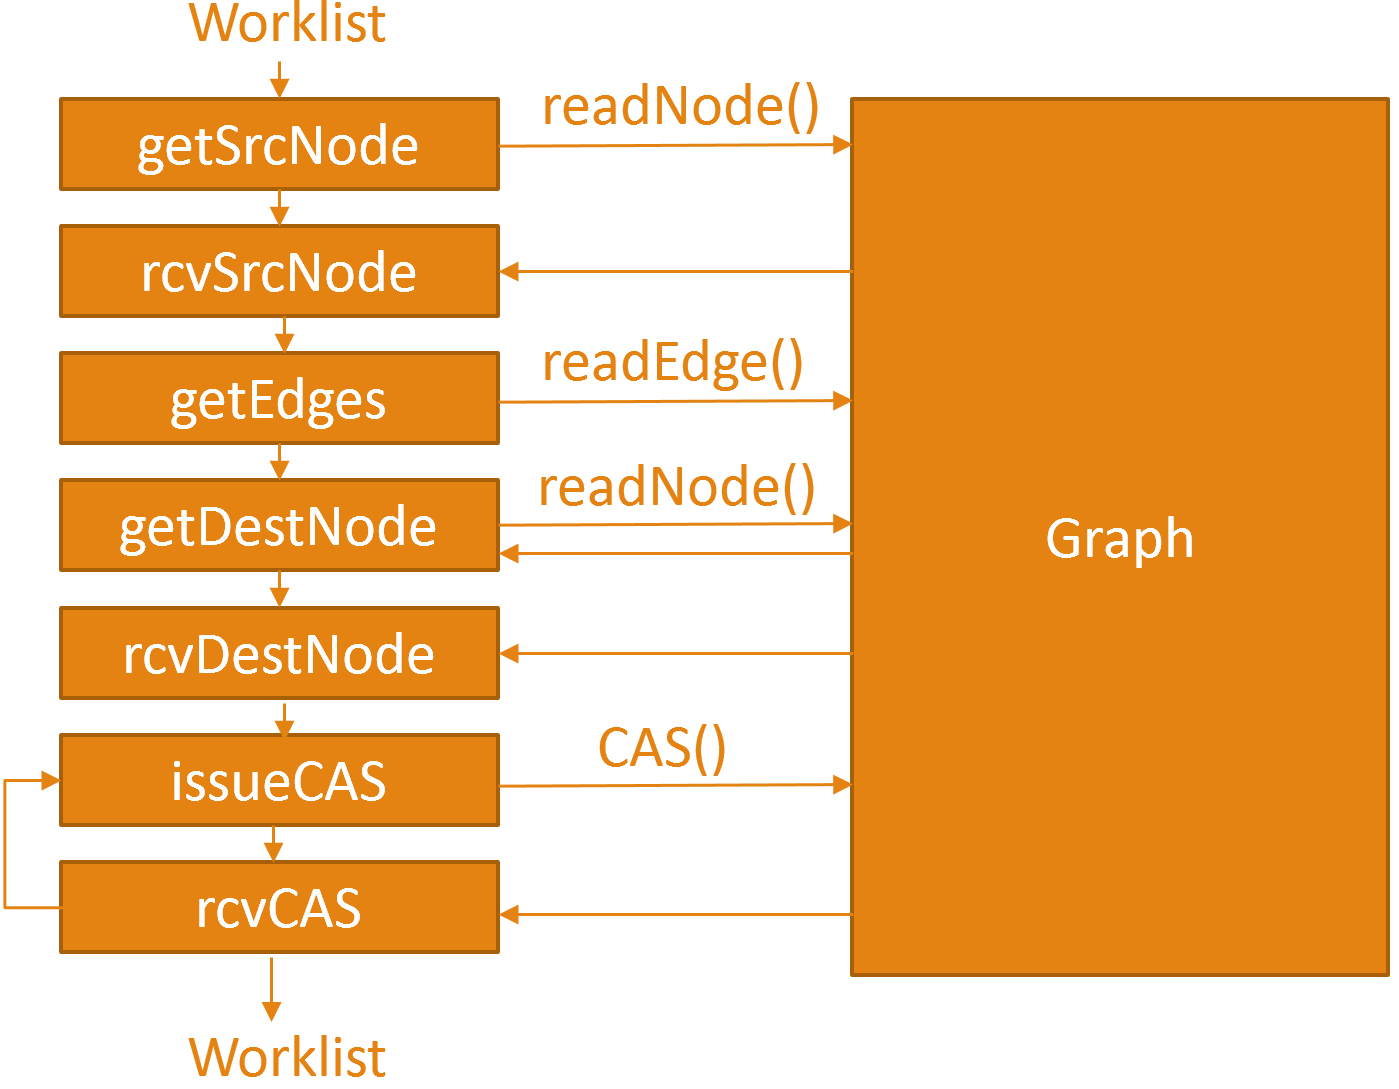
\includegraphics[width=10cm, keepaspectratio]{pics/ssspEngine.png}
\caption{Scheduled SSSP Pipeline}
\label{fig:ssspEngine}
\end{figure}

To generate the engine for SSSP, I manually performed the role of the Galois HLS compiler by scheduling the source 
code into the optimal pipeline stages and generating the requisite scaffolding. Since transactional memory support is 
in the process of being developed by my labmate Xiaoyu Ma, I chose to use a modified version of SSSP with a 
non-atomic \textbf{foreach} with explicit synchronization through the use of the atomic compare-and-swap operation. 
To maximize throughput, the compiler must support multiple Graph method calls in flight; to do this, a simple 
mechanical code transformation is necessary, shown in Figure \ref{fig:ssspSourceCASxform}. By decoupling the method 
request and response calls, the compiler can now schedule the request and response calls into different pipeline 
stages and generate the appropriate context buffering to support multiple calls in flight. The final schedule is 
shown in Figure \ref{fig:ssspEngine}, along with the decoupled Graph request and response calls.

Note that since there are loops in the pipeline, special care must be taken to prevent deadlock, which can occur when 
a thread needs to loop back but the context buffer is full. Since looping back is performed by enqueueing a thread 
context from the end of the pipeline to an earlier stage, this causes deadlock as that thread prevents other threads 
from making forward progress. I solve the deadlock issue through a credit-based system. All threads attempting to 
enter the loop must first reserve space in the context buffer. If no space exists, then the thread stalls until a 
thread has finished looping.

\subsection{Implemented Worklist}

\begin{figure}
\centering
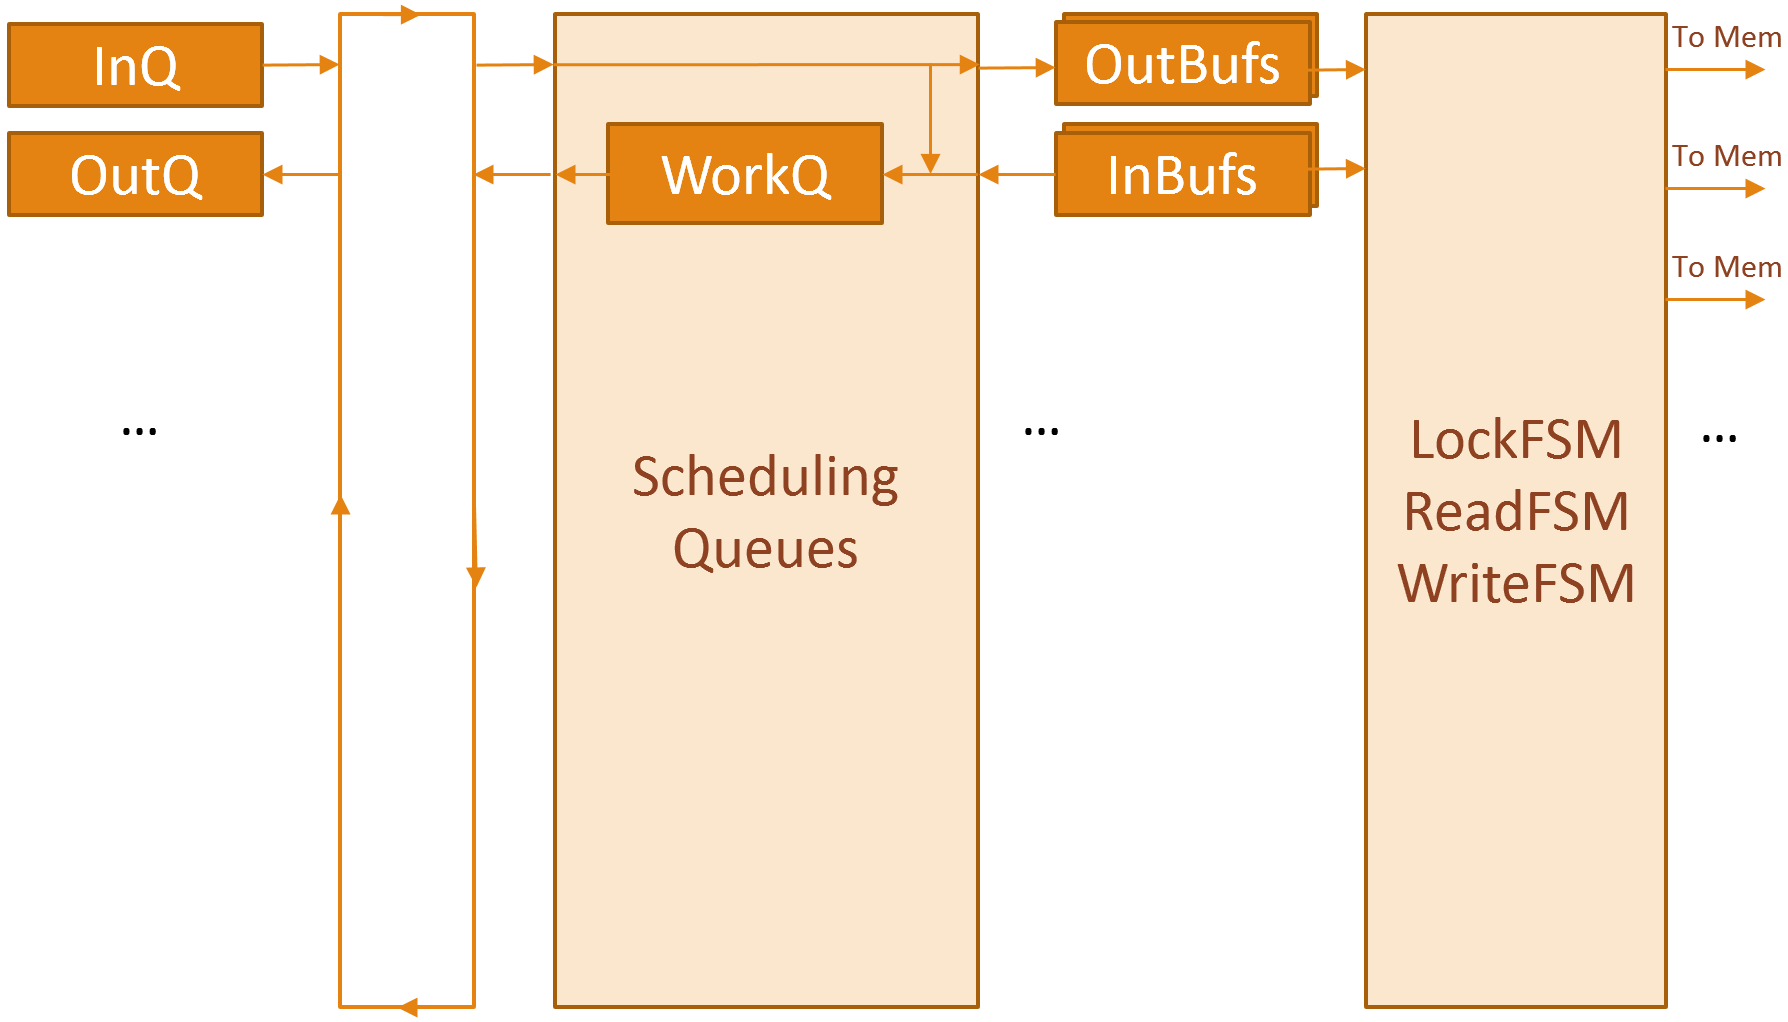
\includegraphics[width=10cm, keepaspectratio]{pics/worklist.png}
\caption{Worklist Microarchitecture}
\label{fig:worklist}
\end{figure}

\begin{figure}
\centering
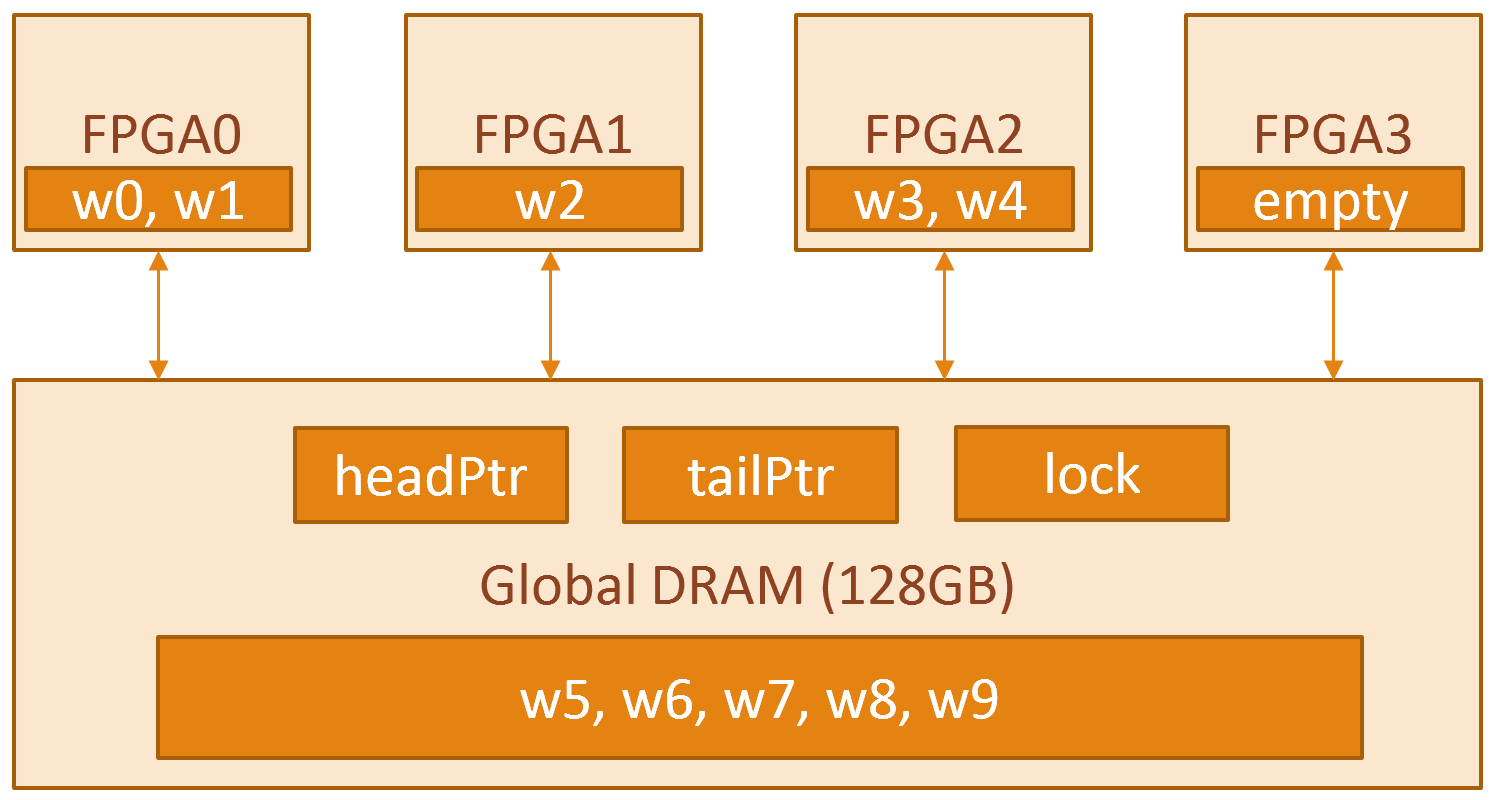
\includegraphics[width=10cm, keepaspectratio]{pics/worklistMem.png}
\caption{Worklist Data Organization Example}
\label{fig:worklistMem}
\end{figure}

For my initial worklist implementation shown in Figure \ref{fig:worklist}, I focused on designing a simple 
microarchitecture capable of scaling to a large (\~16) number of engines. The worklist is comprised of two components, 
the front-end and back-end. The front-end is responsible for work balancing across engines and implementing any 
partial priority ordering schemes specified by the user. The worklist presents a simple packet enqueue/dequeue 
interface to each engine, where each packet currently consists of a single worklist work item. The back-end handles 
worklist spills and fills to main memory.

The worklist front-end consists of \textit{N} lanes, where each lane is connected directly with the engine. Currently, 
only FIFO work ordering is supported. Each lane has a dedicated large-capacity queue (currently 2048 entries). As work 
is generated dynamically under the Galois programming model, I have implemented a work stealing ring network optimized 
for FPGA routability and fast work distribution. If an engine wishes to dequeue a worklist packet but none are 
available, the worklist sends a work steal request to its neighbor. The next time the neighbor performs a worklist 
enqueue, the packet is delivered to the requestor's work stealing queue.

When a worklist front-end lane attempts to perform an enqueue but its work queue is full, it sends the packet to the 
back-end. The back-end contains dedicated per-lane input and output double buffers to stream work items to and from 
global memory. When an output buffer is filled, the data write FSM is triggered. As shown in Figure 
\ref{fig:worklistMem}, global memory contains a unified work queue shared among all FPGAs in the system. The unified 
work queue handles work distribution between FPGAs, enables unbounded work generation, and enables each FPGA to store 
only a small percentage of work items in local BRAM. The FSM therefore locks the global unified work queue before 
writing to the queue. To minimize locking overhead, the FSM performs a streaming write operation consisting of all packets 
in a lane's output buffer (currently 1024). 

The worklist back-end read FSM is triggered when any lane's input buffers are empty and the global work queue is not 
empty. As the FPGA's worklist back-end contains a stale copy of the global worklist head and tail pointers, the 
readFSM will poll the worklist to determine if new work has been added. Like the write FSM, the read FSM locks the 
global work queue before removing entries from the queue.

\subsection{Implemented Graph}

As my labmate Xiaoyu Ma is in charge of implementing transactional memory, for the purposes of evaluating SSSP I have 
only implemented the readNode, readEdges, and compare-and-swap operations. Each operation is implemented as a pipeline 
supporting many concurrent operations in flight. Right now, as shown in Figure \ref{fig:ssspEngine}, the compiler 
instantiates a dedicated graph operation pipeline for each engine graph call. The compiler must then properly bind the 
pipeline memory requests to memory channels. With 16 engines and 16 memory channels, the compiler simply needs to map 
each engine's pipeline requests to a single memory channel. However, with 8 engines or 4 engines, the compiler must 
map more than one memory channel to a single engine's graph requests. Proper care must be taken to balance memory 
channel utilization to achieve high performance while satisfying FPGA routing constraints.


\subsection{SSSP Simulated Results}


\begin{table}
\centering
\begin{tabular}{ | l | l l | l | l | l | l |}
  \hline
  \textbf{Module} & \textbf{Slices} & \textbf{\% of total} & \textbf{Slice Reg}  & \textbf{LUTs}  & \textbf{BRAM} \\
  \hline
  XC6VHX565T & 88,560 & 100\% & 708,480 (100\%) & 354,240 (100\%) & 912 (100\%)\\
  \hline
  Convey Top & 67,586 & 76\% & 198,903 (28\%) & 182,824 (51\%) & 146 (12\%)\\
  \hline
  * BSV Wrapper & 33,979 & 38\% & 88,601 & 68,060 & 96 \\
  \hline
  ** SSSP Top & 20,831 & 24\% & 50,816 & 46,617 & 80 \\
  \hline
  *** SSSP Engines & 3,036 & 3.4\% & 8,796 & 7,916 & 24 \\
  \hline
  *** Graph & 5,576 & 6.3\% & 15,862 & 13,262 & 24 \\
  \hline
  *** Worklist & 4,491 & 5.1\% & 9,420 & 10,291 & 32 \\
  \hline
  **** Worklist Backend & 3,629 & 4.1\% & 7,650 & 8,334 & 24 \\
  \hline
\end{tabular}
\caption{SSSP FPGA Resource Usage (4 engines)}
\label{table:ssspResourceUsage}
\end{table}

\begin{table}
\centering
\begin{tabular}{ | l | l |}
  \hline
  \textbf{FPGA Count} & 4\\
  \hline
  \textbf{Engine Count per FPGA} & 4\\
  \hline
  \textbf{Clock Speed} & 125MHz\\
  \hline
  \textbf{Graph Mem Ops in Flight per Port} & 128\\
  \hline
  \textbf{Worklist Entries per Engine} & 8192\\
  \hline
  \textbf{Engine Double Buffer Size} & 1024\\
  \hline
\end{tabular}
\caption{SSSP uArch Tested Configuration}
\label{table:ssspConfig}
\end{table}

\begin{figure}
\centering
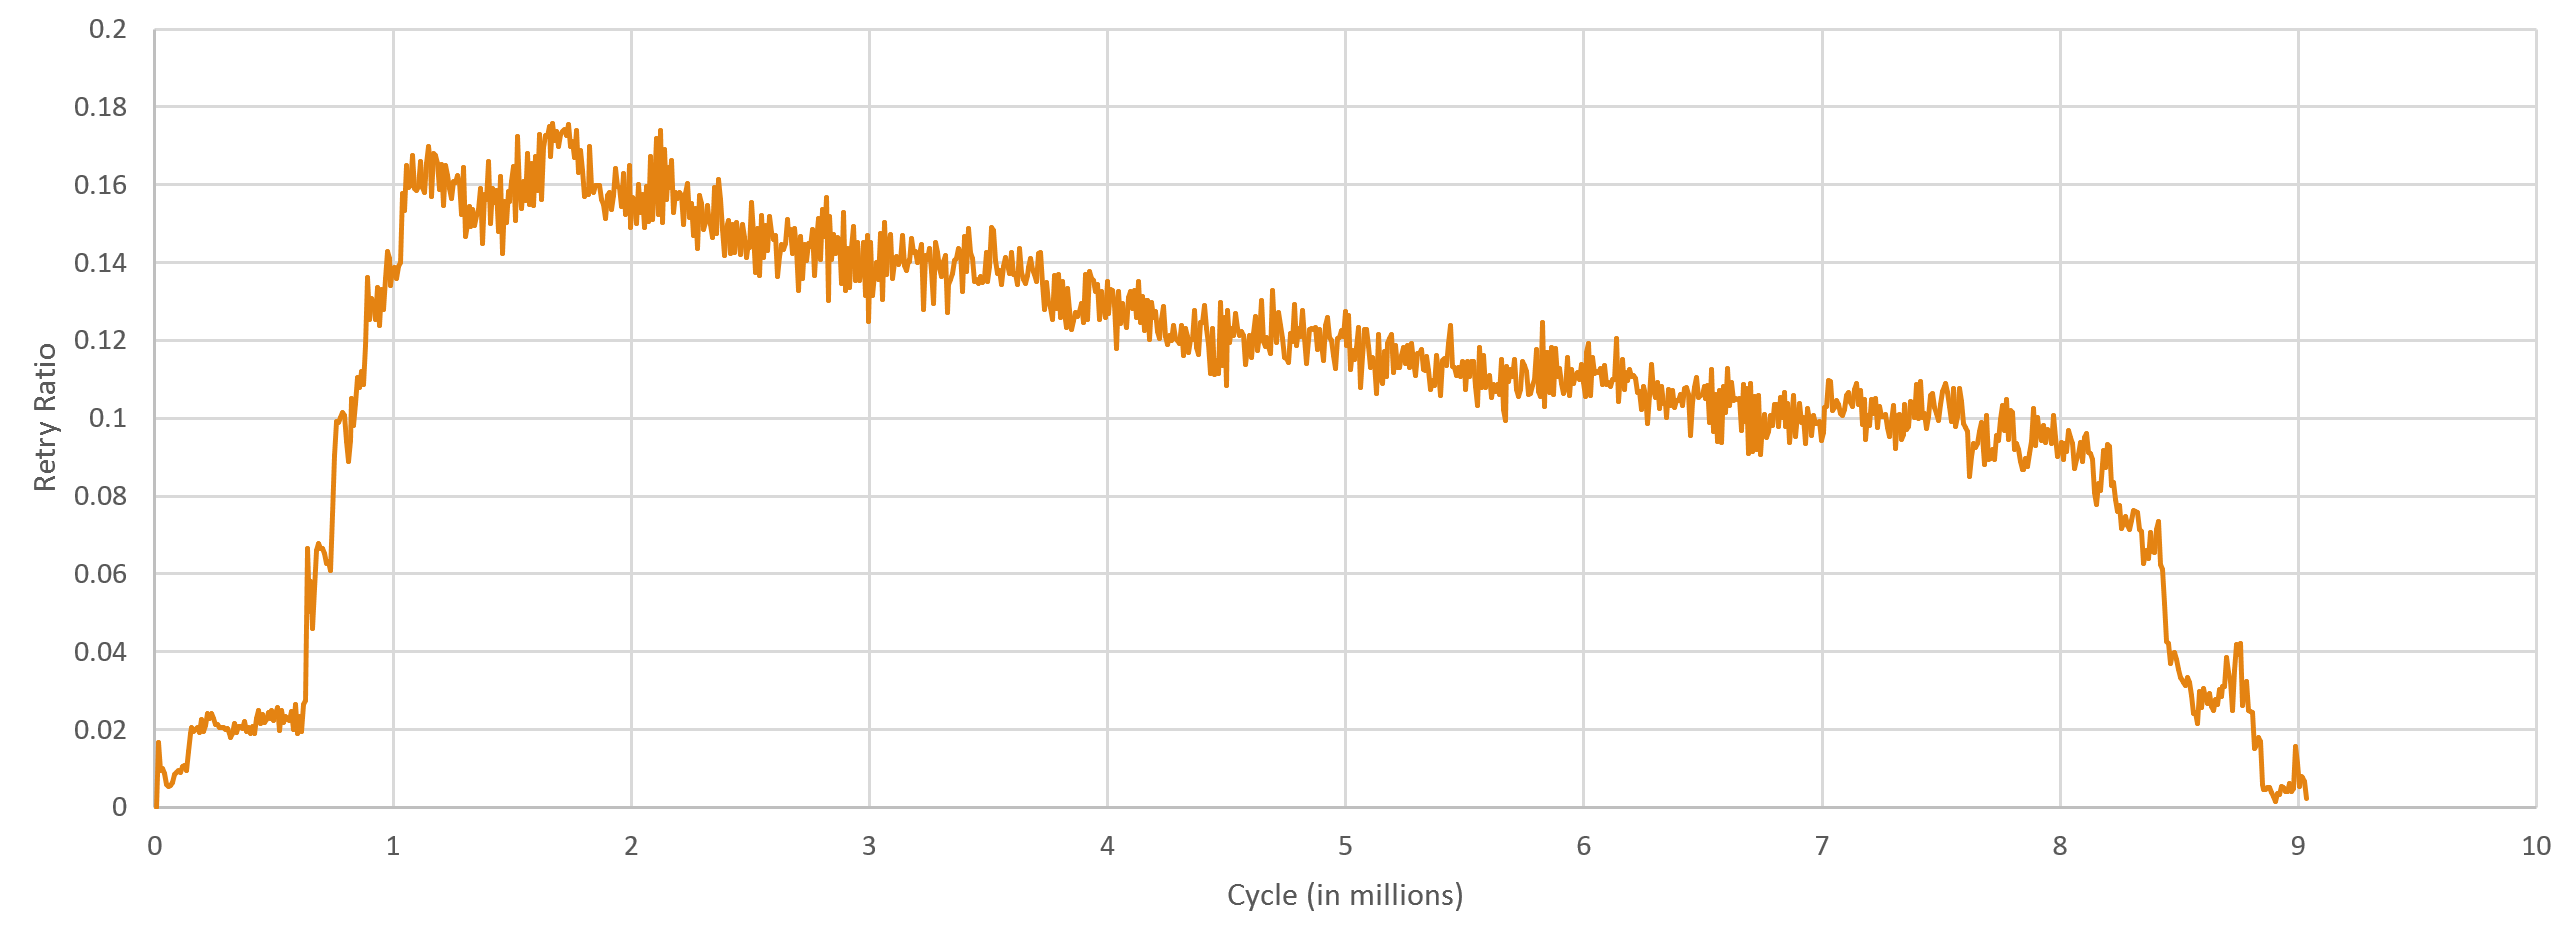
\includegraphics[width=15cm, keepaspectratio]{pics/casretry.png}
\caption{Compare-and-Swap Retry Ratio}
\label{fig:casretry}
\end{figure}

\begin{figure}
\centering
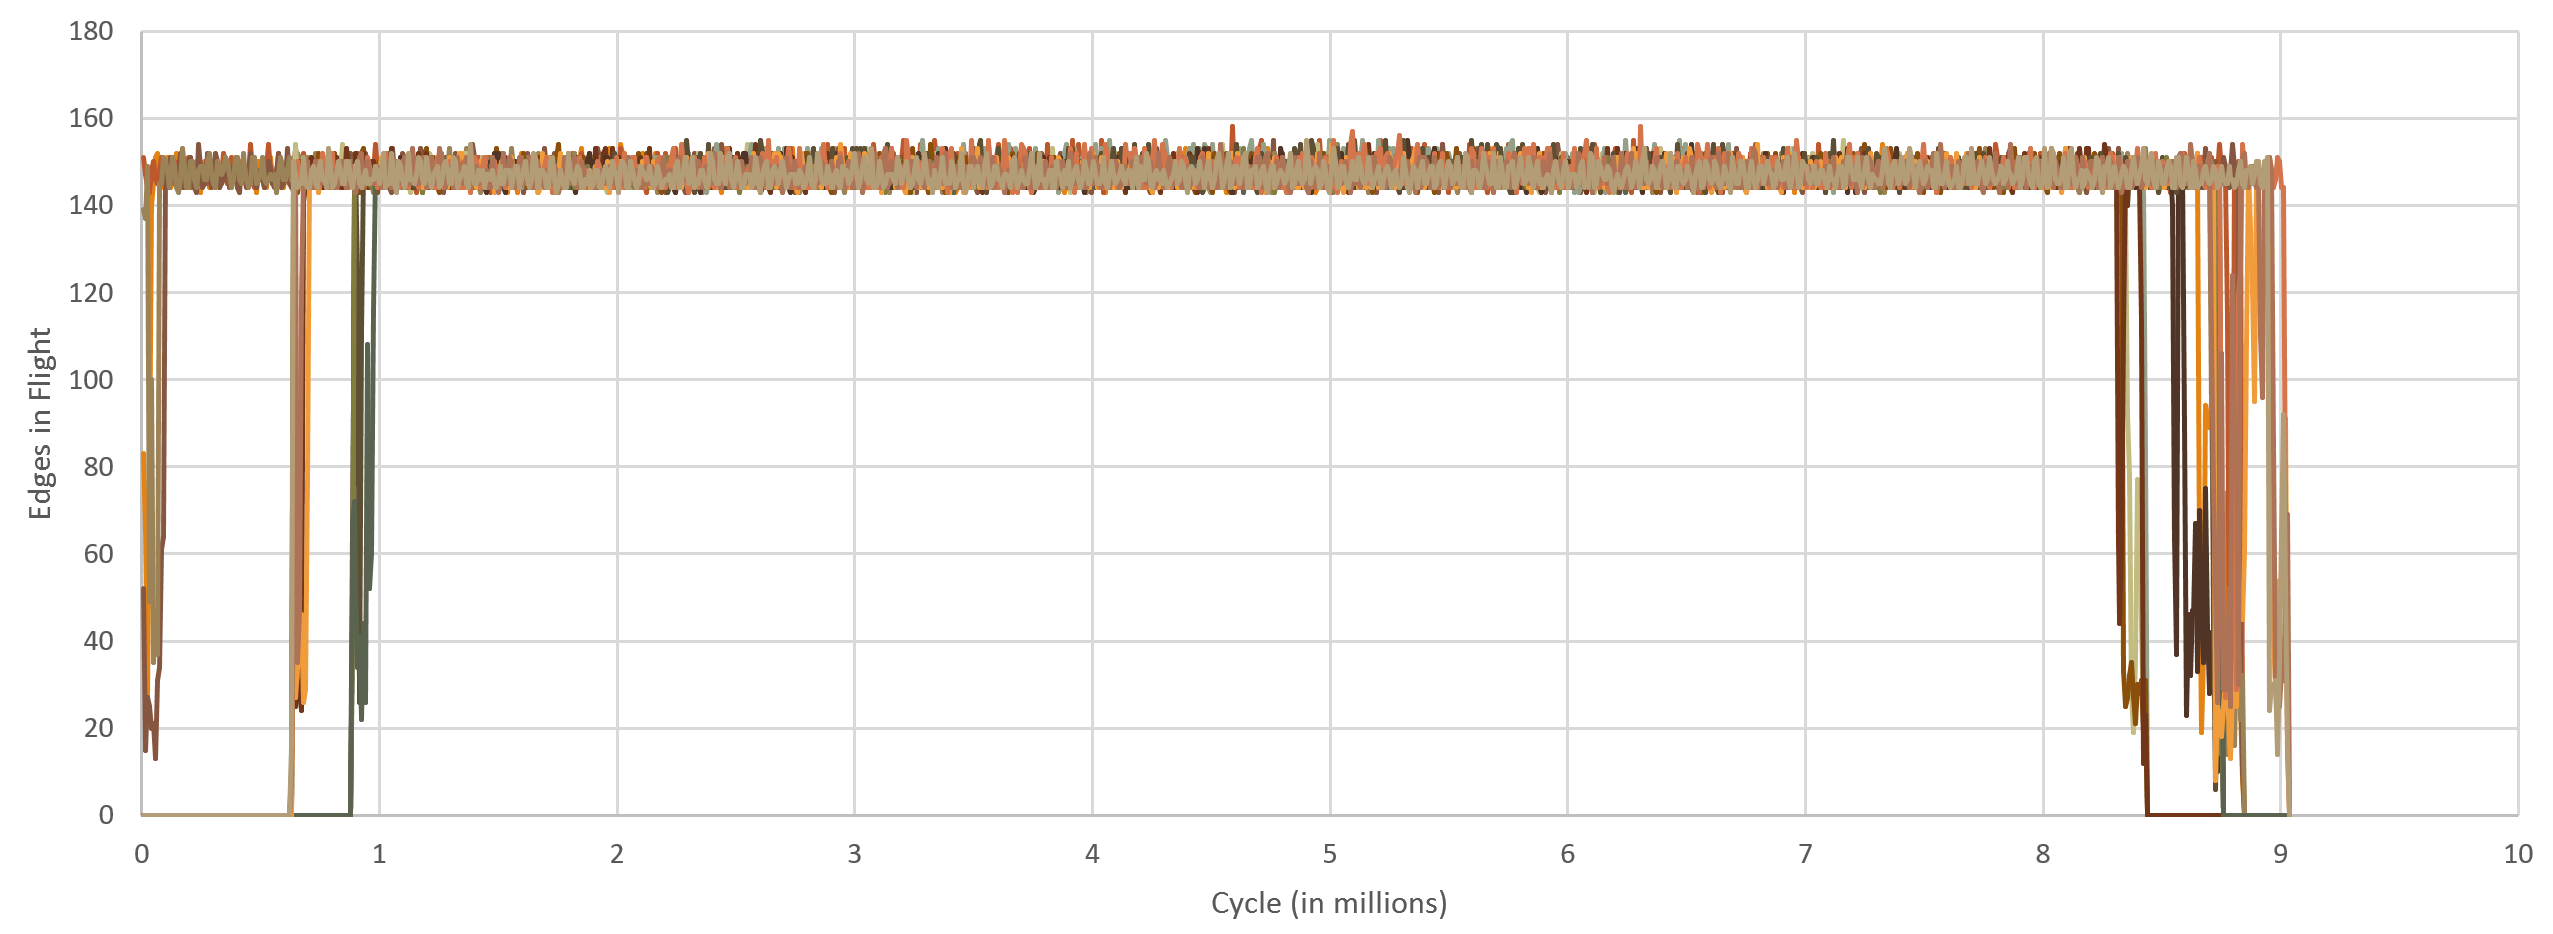
\includegraphics[width=15cm, keepaspectratio]{pics/edgesInFlight.png}
\caption{Edges in Flight per Engine}
\label{fig:edgesInFlight}
\end{figure}

\begin{figure}
\centering
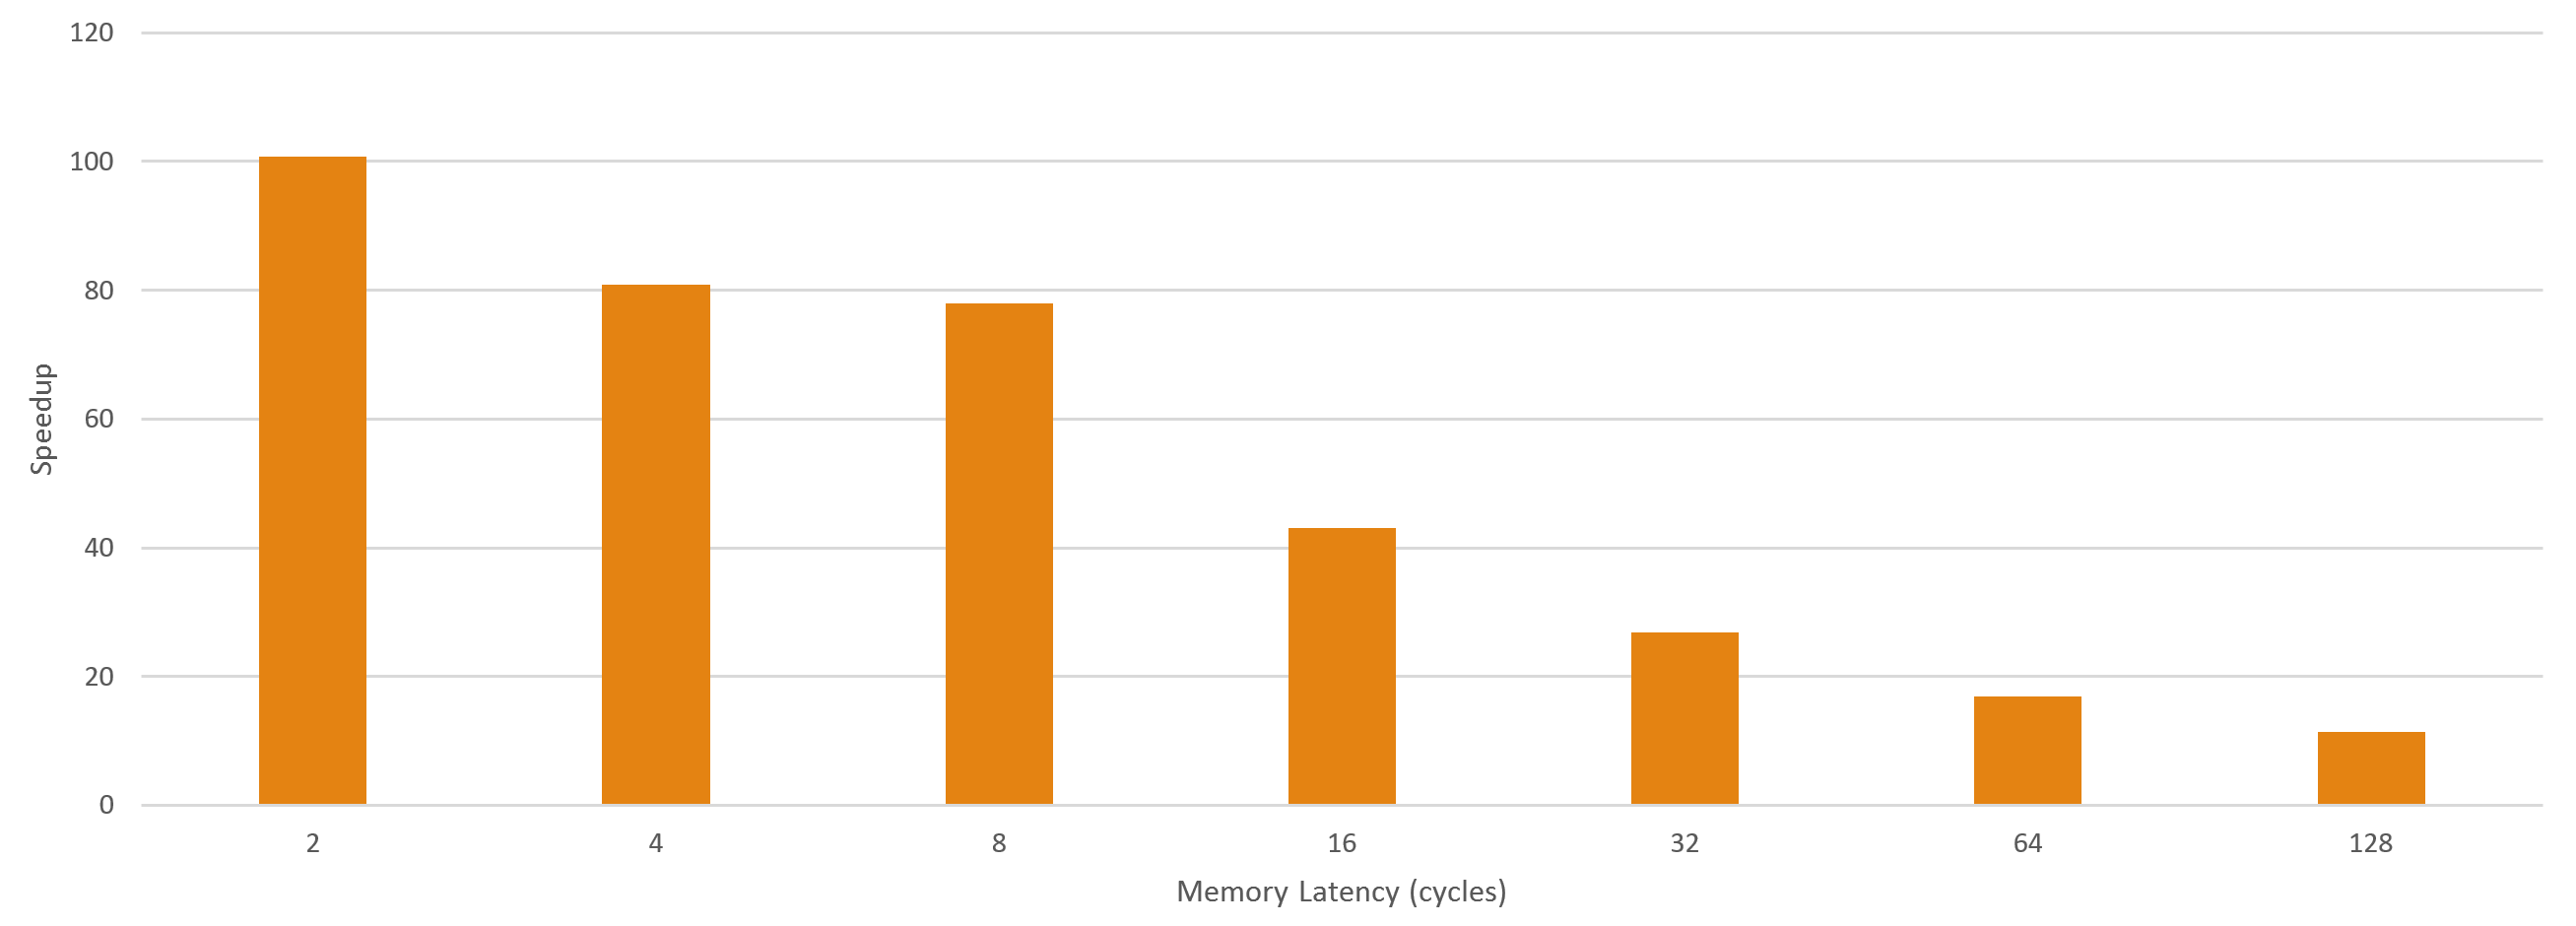
\includegraphics[width=15cm, keepaspectratio]{pics/speedup.png}
\caption{Edges Committed per Second Speedup vs. Software}
\label{fig:speedup}
\end{figure}

I was able to successfully synthesize a 4-engine SSSP microarchitecture. The FPGA bitfile is programmed to all four 
Convey Application FPGAs, resulting in 16 engines in total. The details of my configuration are shown in Table 
\ref{table:ssspConfig}. With up to 128 memory operations in flight per memory port, the design should in theory be able 
to send a memory request to each channel every cycle, resulting in up to 16 memory requests per cycle. FPGA resource 
utilization is shown in Table \ref{table:ssspResourceUsage}. Convey overheads are high: the Galois microarchitecture 
is only 32\% of the size of the entire design, consuming 24\% of total slices in the FPGA. The Bluespec wrapper itself 
uses 14\% of available FPGA slices; additional engineering effort will be required to minimize this. Unfortunately, I 
am currently unable to meet timing at 150MHz. Instead, the Galois microarchitecture is downclocked to 125MHz while 
the rest of the Convey infrastructure runs at 150MHz. 

Although I was able to synthesize my design, I have so far been unable to run on hardware due to some minor technical 
issues. However, I am able to run reasonably-sized graphs to completion in the Bluesim simulation framework. The SSSP 
design is functionally correct compared to a software golden model. For my tests, I used USA-road-NY, an undirected 
graph consisting of all roads in the state of New York, containing 264K nodes and 730K edges. However, this graph is 
too small to obtain any meaningful result running in software. As a rough approximation to overall performance, I 
measured the rate at which the SSSP engines were able to commit SSSP destination nodes. A commit occurs when a shorter 
path has been discovered, resulting in a distance update to the destination node and the destination node being added 
to the worklist. I then measured the average edges committed each second by a single-threaded Galois software 
implementation running a large workload (USA-road-USA) on a 4-socket Xeon E7540 server.

The results in Figure \ref{fig:speedup} shows the potential of the Galois microarchitecture, but also its current 
limitations. Although I can achieve 80x to 100x speedup with 2-8 cycles of memory latency, performance drops 
significantly as memory latency is swept from 16 to 128. This is due to the microarchitecture being immature; I believe 
that the issue lies with the number of memory round-trips required to synchronize and begin a worklist spill or fill 
operation. The current worklist spills to a global shared queue; a simple optimization would be to split the global 
shared queue into private queues and perform dynamic work balancing.

To preserve atomicity, SSSP node distance updates are made using the atomic compare-and-swap operation. Figure 
\ref{fig:casretry} shows the number of CAS retry operations as a function of time across the entire span of program 
execution. Retries start out low, but quickly ramp up as multiple engines are assigned work by the scheduler. The 
retry ratio peaks after all engines are warmed up and executing, and gradually decreases as each engine starts 
processing nodes further away from other engines. The small spikes near the end of execution are a result of better 
paths being discovered, resulting in idle engines being woken up and causing more conflicts.

Figure \ref{fig:edgesInFlight} shows the number of edges in flight per engine as a function of time. After each FPGA 
has been woken up, a steady state of roughly 150 edges in flight is quickly reached and remains there for the entire 
duration of program execution. This demonstrates that there is sufficient parallelism in the algorithm and input 
dataset, which enables high performance from the throughput-optimized Galois microarchitecture.
